\section{Results}

\myparagraph{Validation} 
After the preprocessing steps have been built, they have been validated on the previous analyses already performed, the first being Peri-Stimulus Time Histogram (PSTH). The spike trains used to produce the PSTH come from the recordings of all neurons 5 seconds before and after the \emph{lift} landmark. 
\begin{figure}[h!]
	\centering
	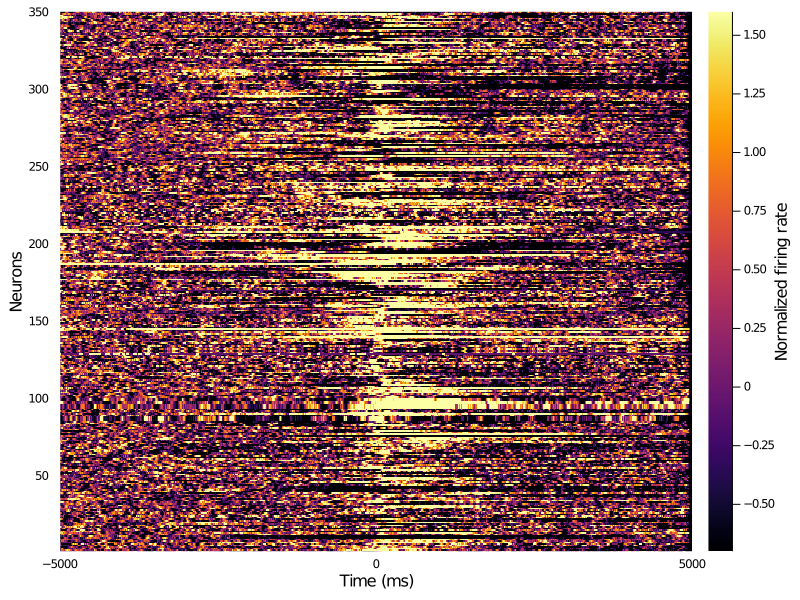
\includegraphics[scale=0.5]{../../plots/psth.pdf}
	\caption{Normalized peri-event histogram}
	\label{fig:psth}
\end{figure}
They have been averaged by trials, and convolved with a $\sigma=10$ gaussian kernel, and normalized using the firing rates between 5 and 3 seconds before the landmark. To give an example of the framework built to deal on the data, this is the code used to generate the data:
\begin{lstlisting}[frame=single]
spiketrains = slice(data.t, data.lift, around=[-5000, 5000], 
			convolution=true, normalization=true, 
			average=true, over=[-5000, -2000])
\end{lstlisting}


After PSTH, it has been performed one more analysis, to validate that convolution was working properly. It consisted in calculating the correlation coefficient of the convoluted signals of neighbor vs distant neurons around landmarks, and you can see the results in Figure \ref{fig:corr-coeff}.

\begin{figure}[h!]
	\centering
	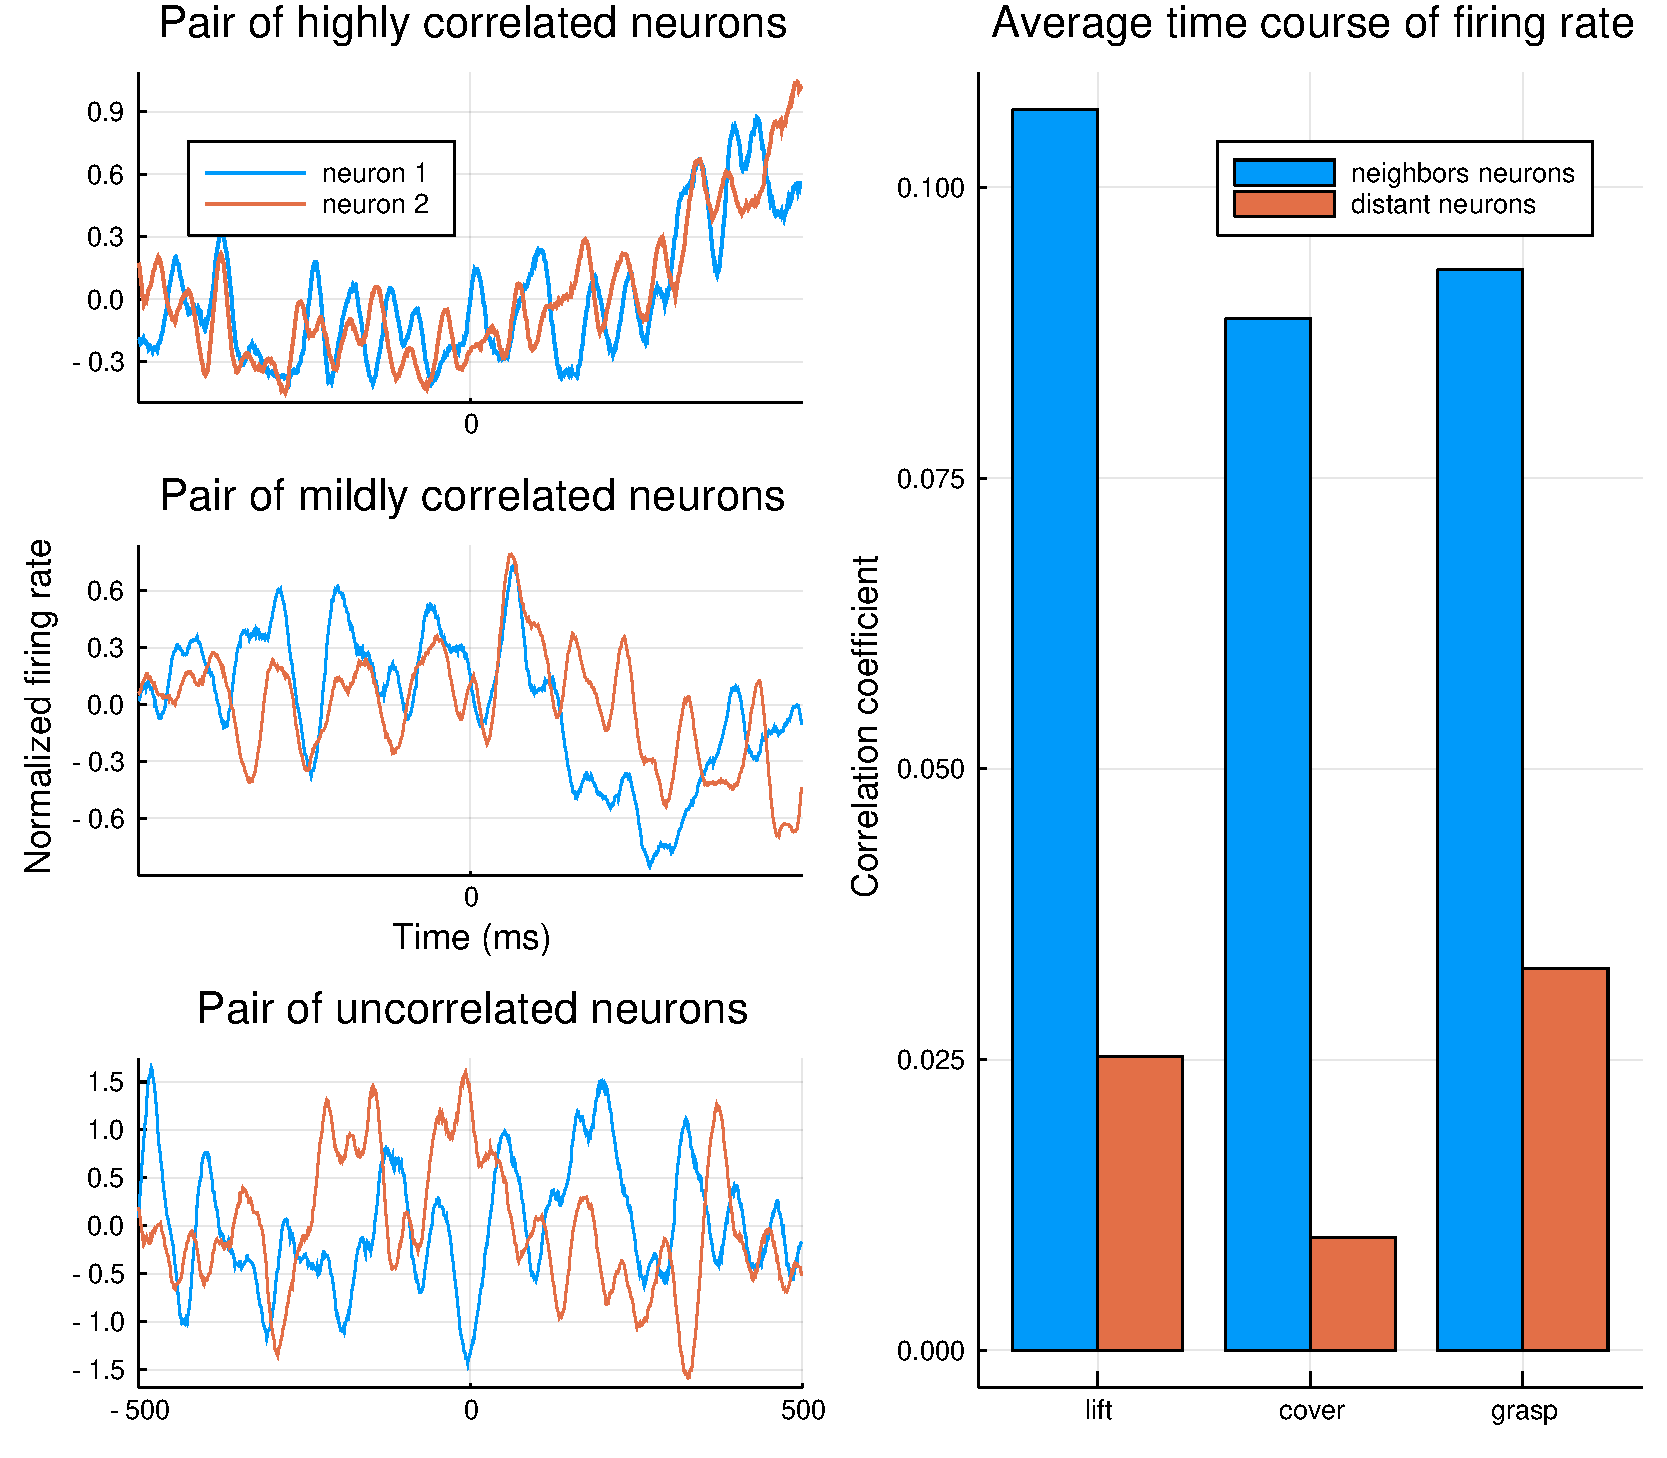
\includegraphics[scale=0.5]{../../plots/corr-coef.pdf}
	\caption{Firing time course around lift for pairs of neighbouring cells and correlation of average time course firing rate of neighbour vs distant nerons}
	\label{fig:corr-coeff}
\end{figure}

\myparagraph{PCA} 

The first novel analysis performed on the data was PCA.	Before applying it, the data has been convoluted with a gaussian kernel with $\sigma=10$, normalized using the activity of 500ms before and after the landmark, and at last averaged across trials, for the reasons explained above.
\begin{figure}[h!]
	\centering
	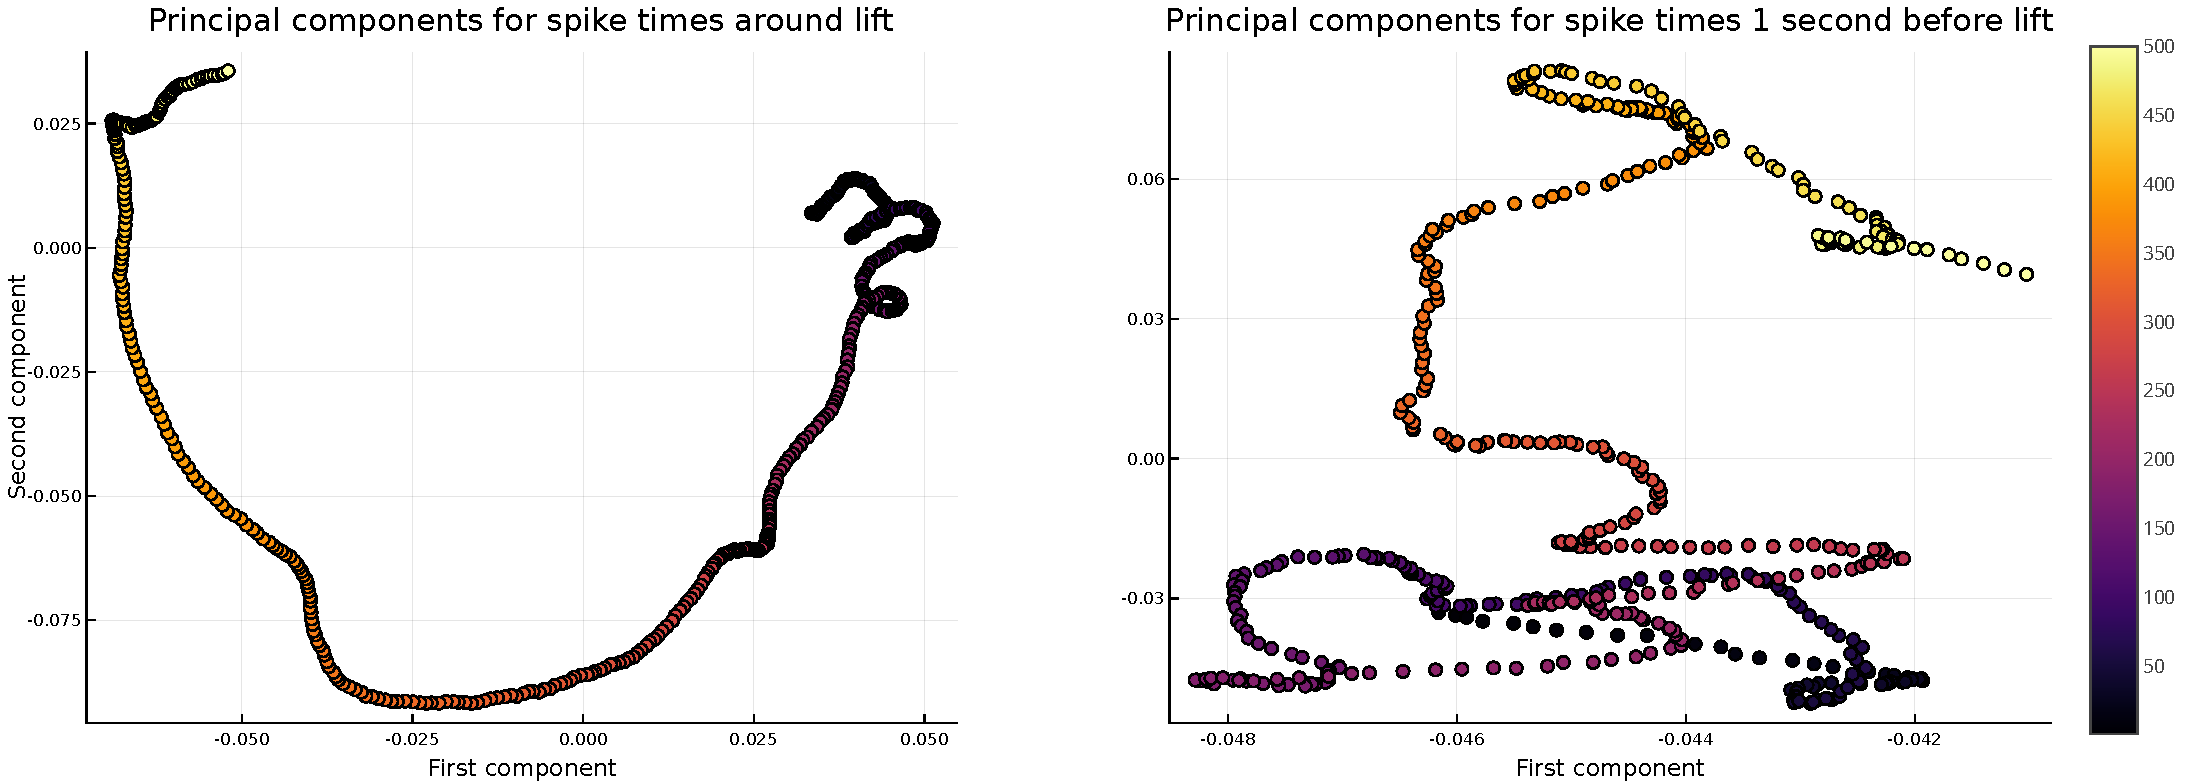
\includegraphics[width=6in]{../../plots/pca-lift-vs-non-lift.pdf}
	\caption{Trajectory of the 2 principal components of most active spike trains 250ms before and after lift. 
}
	\label{fig:pca-500}
\end{figure}

The observed trajectory represents \cite{cunningham2014dimensionality} how the small population of neurons recorded encodes the arm lifting. It is noticeable a circular trajectory, as it is found in the motor and premotor cortex \cite{churchland2012neural}. 
Each point represents the direction of maximum variance in the data for any given feature, that in this case means at any time point. 
% Hence, the plot can be interpreted by observing that, to maximise the variance, PCA projects the beginning and the end of the time series on opposite sides of the spa 

It is important to remark that this kind of trajectory is not found when applying PCA on other time points, where the rats were not performing the same action simultaneously. For example, Figure \ref{fig:pca-500} (right) shows the pattern plot between 1.5s and 1s before lift.


A further step has been taken in this direction, analysing the differences in the principal components of trials where the interval between \emph{lift} and \emph{cover} was high and were it was low, basically exploring the differences that speed has on the neural trajectory.
It is very interesting to notice that the projections are very close at the beginning, but then they follow almost specular paths.

\begin{figure}[h!]
	\centering
	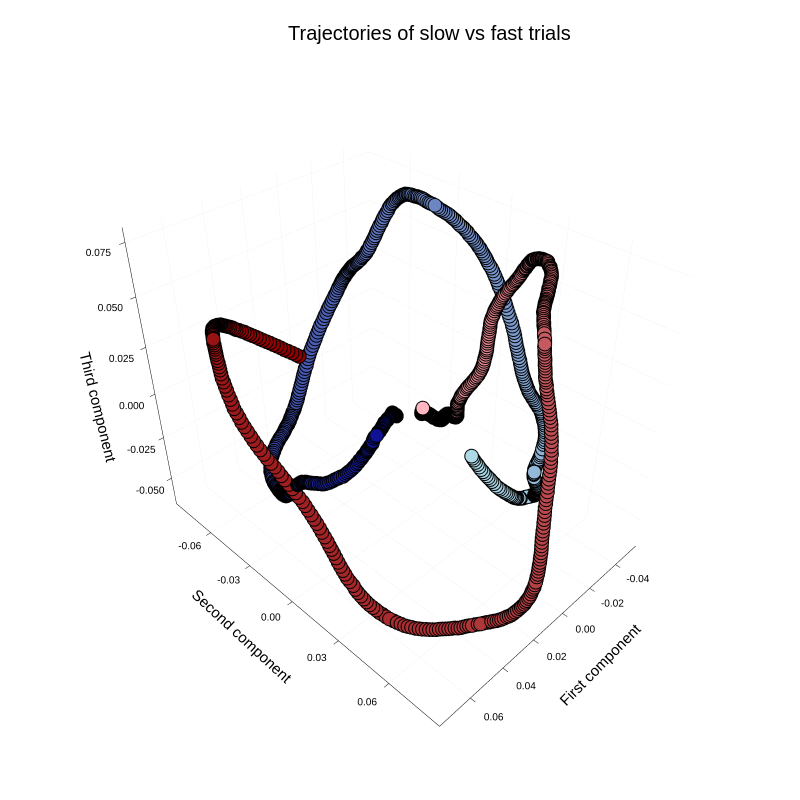
\includegraphics[scale=0.4]{../../plots/pca-speed.png}
	\caption{Trajectory of the 3 principal components between 250ms before and after lift. Trajectory of neural response of faster movements is in red, and in blue for slower movements. Light is the start of a trajectory, dark is the end.}
	\label{fig:pca-speed}
\end{figure}

\myparagraph{Gaussian-Process Factor Analysis} 

GPFA has been applied using the Elephant \cite{elephant18} package for python. It fitted on simultaneous recordings, coming from single trials, and it has been used to visualise them, comparing trials where the rats movement was slow and fast. 
Speed is known to be one of the major features encoded in cerebellum activity \cite{becker2019cerebellar}, yet its not discernible from the trajectories plotted on the GPFA dimensions, as shown in figure \ref{fig:gpfa-speed}.
\begin{figure}[h!]
	\centering
	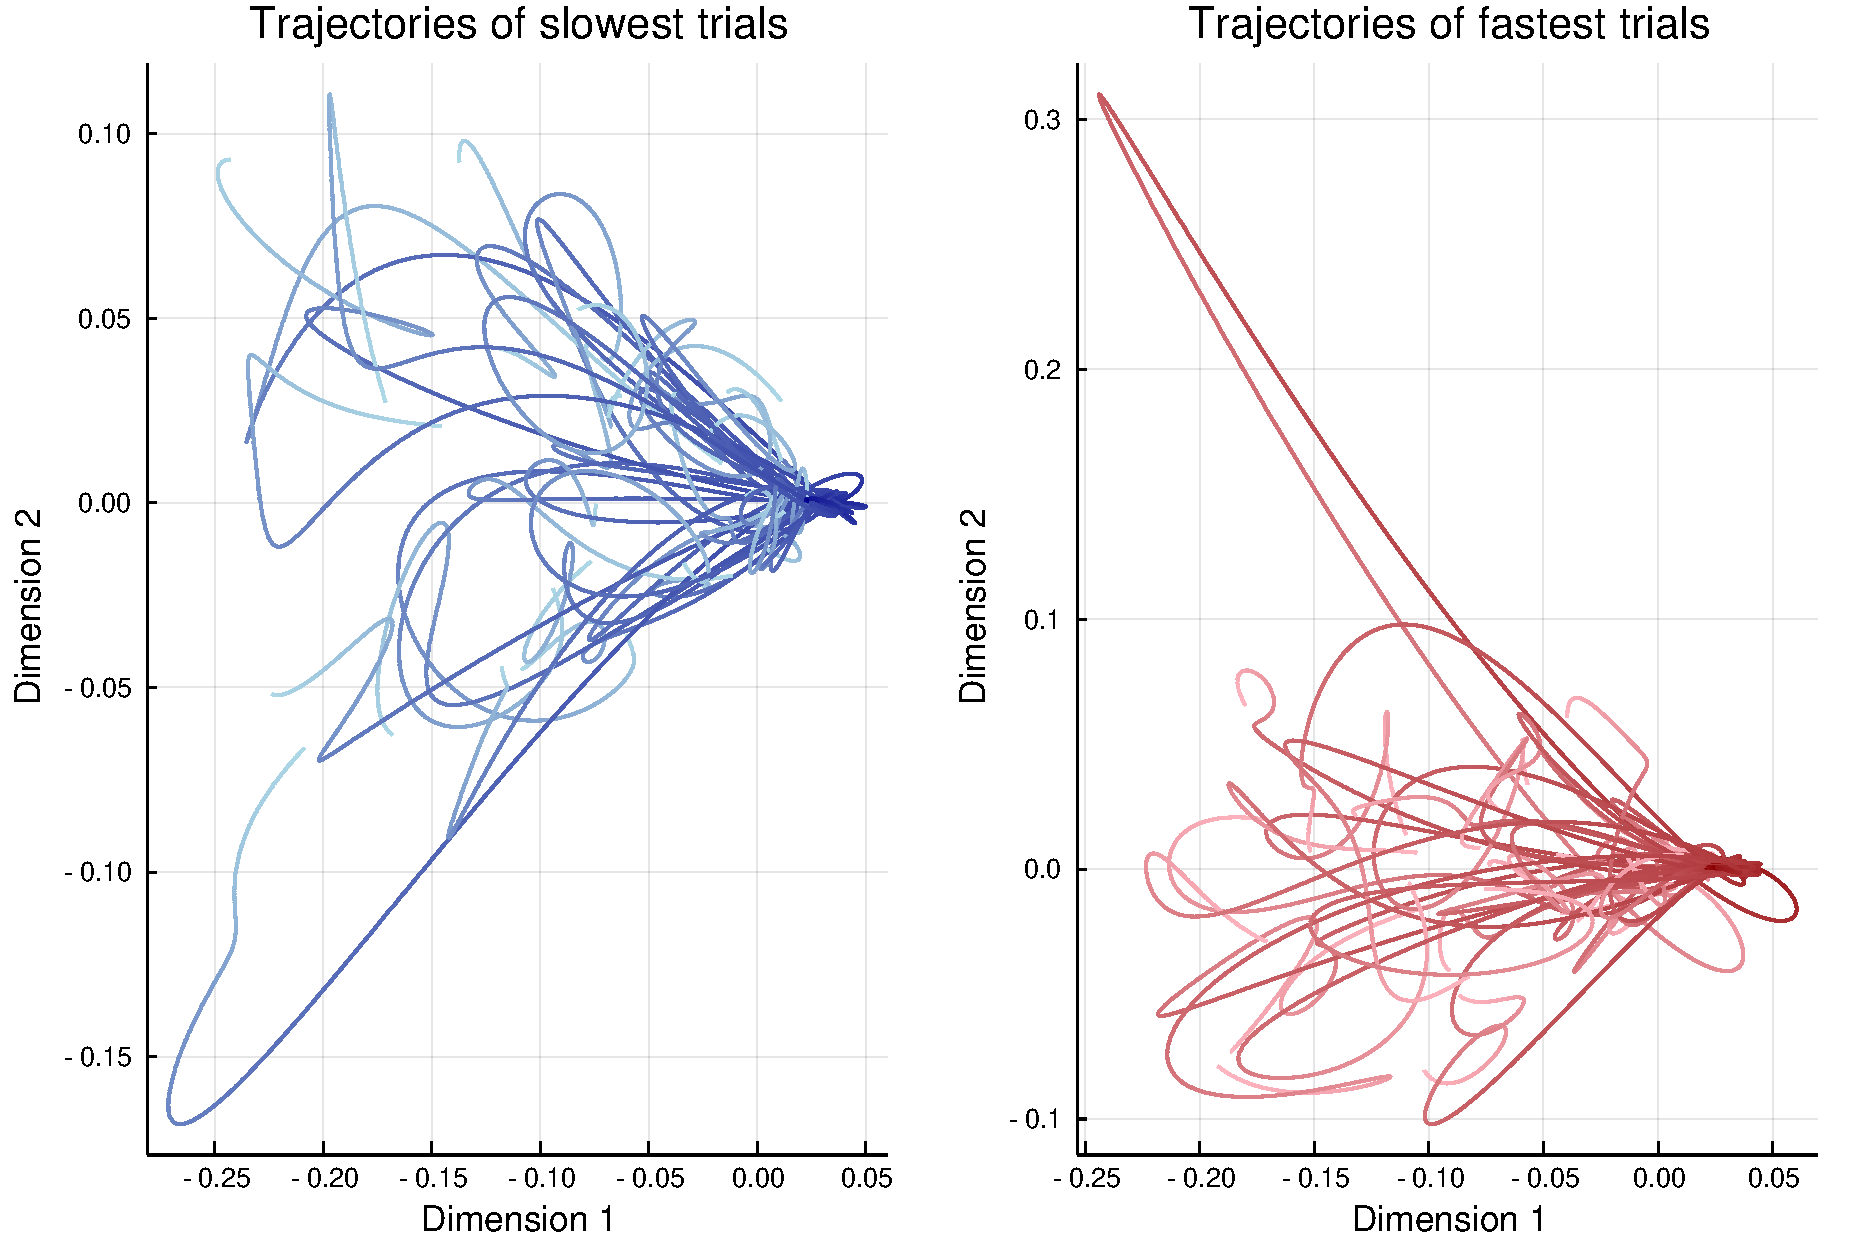
\includegraphics[scale=0.5]{../../plots/gpfa-slow-vs-fast.pdf}
	\caption{Neural trajectories of 5\% slowest (left) and fastest (right) trials}
	\label{fig:gpfa-speed}
\end{figure}
Future work will comprise further preprocessing or data selection, since we expect that in clean data condition a dimensionality reduction technique such as GPFA should capture such an important feature of the data.

% \begin{figure}[h!]
% 	\centering
% 	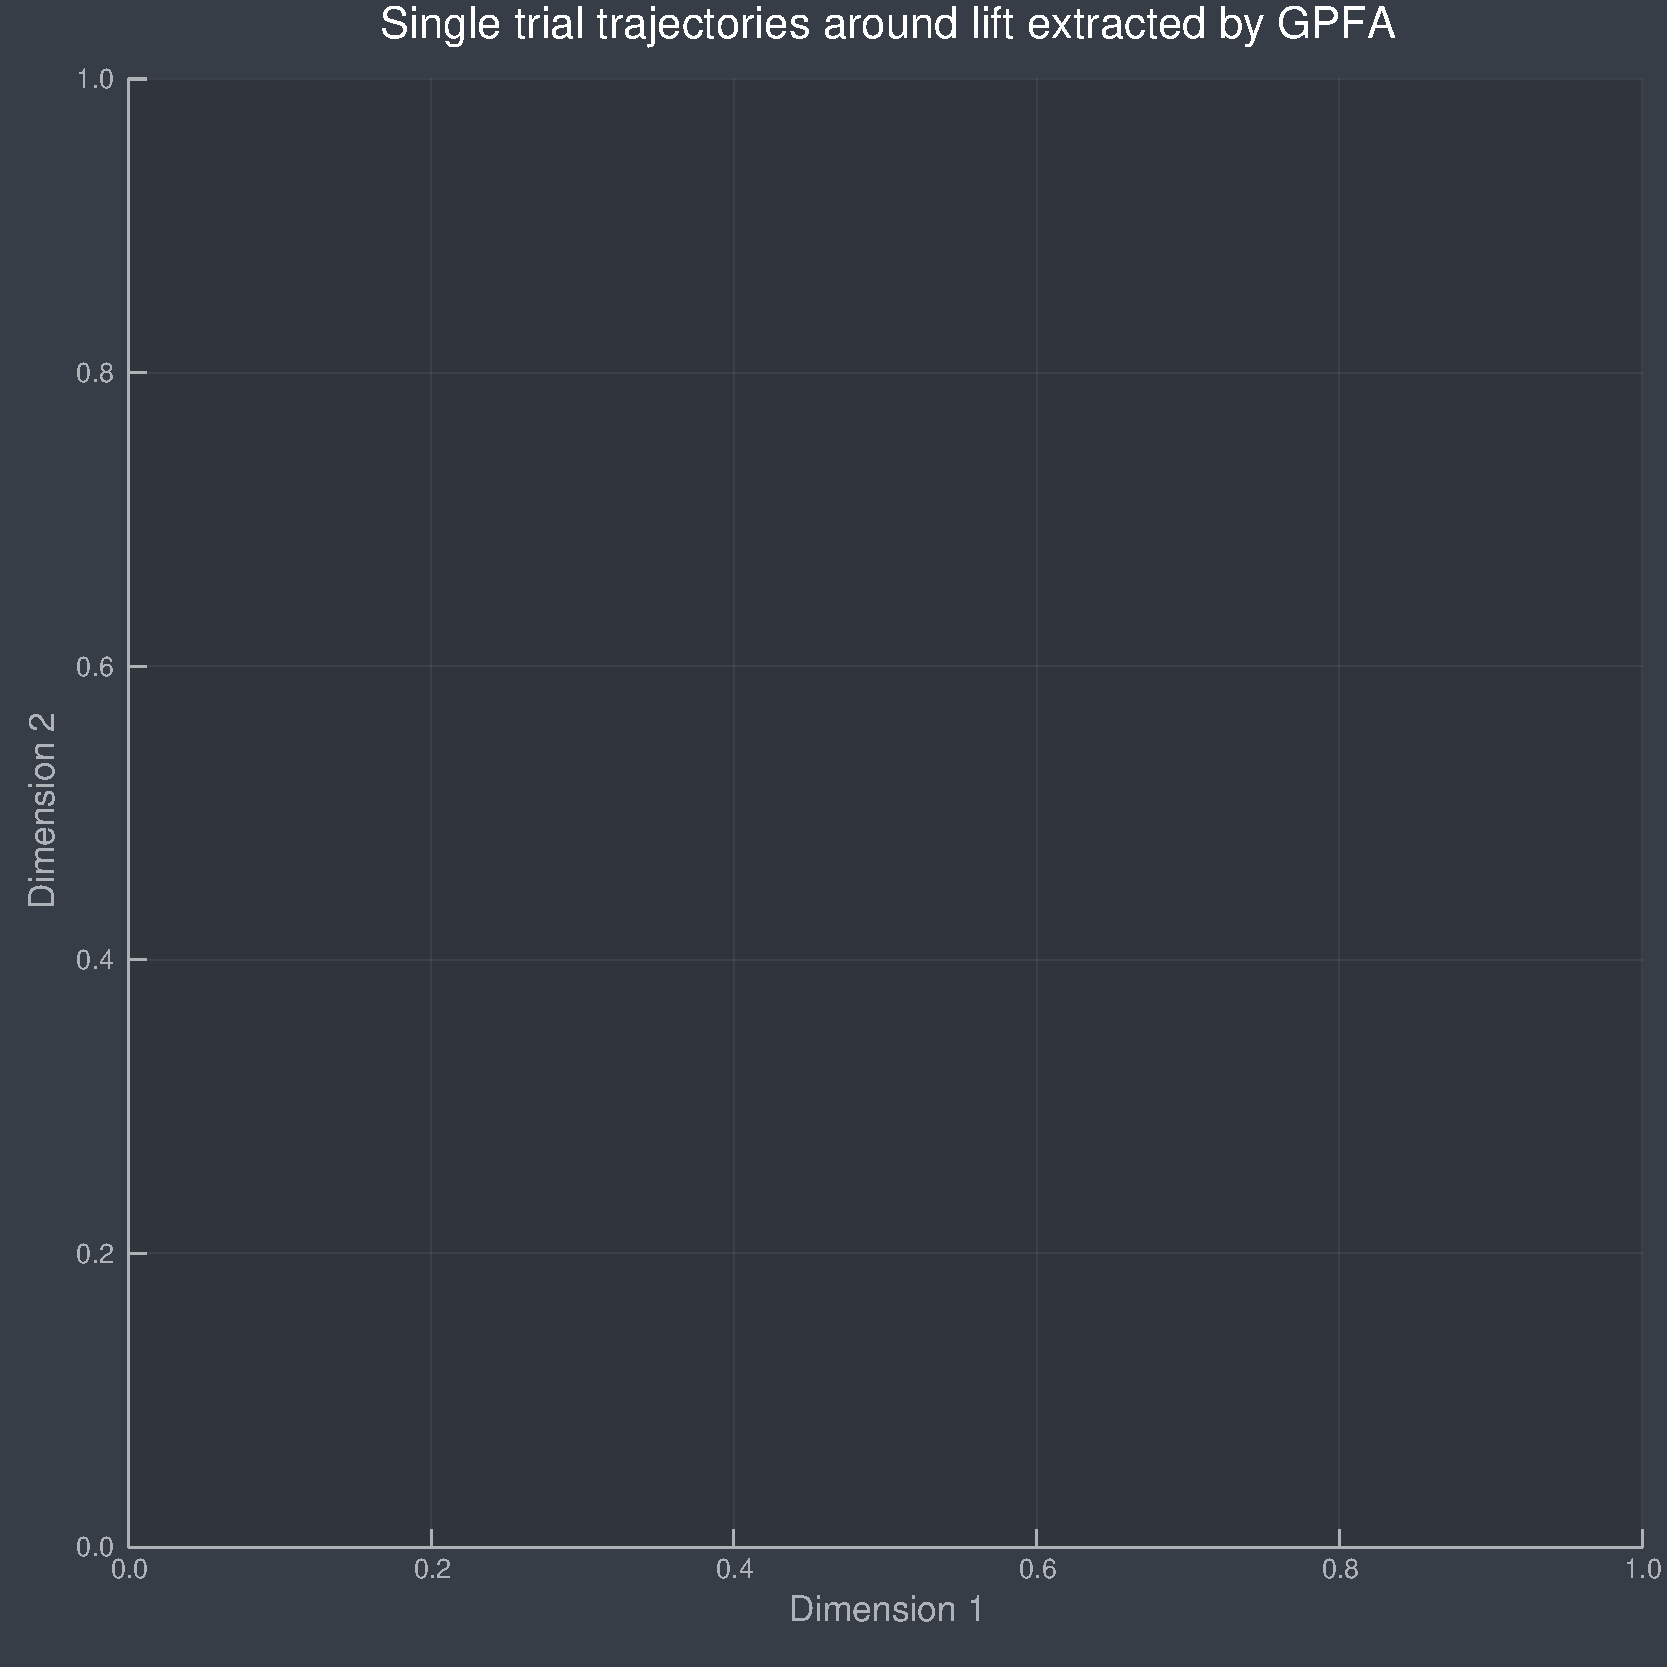
\includegraphics[scale=0.5]{../../plots/gpfa2d.pdf}
% 	\caption{}
% 	\label{fig:gpfa2d}
% \end{figure}



